%  !TeX  root  =  user_guide.tex 
\section{Extension de GeoRaster Oracle}\label{sec:oracleraster}

%In Oracle databases, raster data can be stored in SDO\_GEORASTER objects available with the 
%Oracle Spatial extension. In \qg, the \toolbtntwo{oracle_raster}{Oracle GeoRaster Plugin} 
%is supported by GDAL, and depends on Oracle's Database product being installed and working 
%on your machine. While Oracle is proprietary software, they provide their software free for 
%development and testing purposes. Here is one simple example of how to load raster images 
%to GeoRaster:

Dans les bases de données Oracle, les informations rasters sont stockées au sein d'objets SDO\_GEORASTER disponibles avec l'extension Oracle Spatial. Dans \qg, le support de \toolbtntwo{oracle_raster}{Oracle GeoRaster Plugin} est apporté par GDAL et nécessite l'installation et l'utilisation des produits Oracle sur votre machine. Bien que ces produits soient propriétaires, Oracle les fournit gratuitement dans un but de test ou de développement. Voici un exemple assez simple quant au chargement d'images rasters en GeoRaster :

\begin{verbatim} 
$ gdal_translate -of georaster input_file.tif geor:scott/tiger@orcl
\end{verbatim}

%This will load the raster into the default GDAL\_IMPORT table, as a column named RASTER.
Le raster va être chargé dans la table par défaut, GDAL\_IMPORT, en tant que colonne nommée RASTER.

%\subsection{Managing connections}
\subsection{Gérer les connexions}

%Firstly, the Oracle GeoRaster Plugin must be enabled using the Plugin Manager (see Section 
%\ref{sec:load_core_plugin}). The first time you load a GeoRaster in \qg, you must create a 
%connection to the Oracle database that contains the data. To do this, begin by clicking on 
%the \toolbtntwo{oracle_raster}{Select GeoRaster} toolbar button, it will open the Select Oracle 
%Spatial GeoRaster dialog window. Click on \button{New} to open the dialog window, and specify 
%the connection parameters (See Figure \ref{fig:oracle_create}):

Tout d'abord, l'extension GeoRaster doit être activé dans le gestionnaire d'extension (voir setion \ref{sec:load_core_plugin}). Au premier chargement d'un GeoRaster dans \qg, vous devrez instaurer une connexion vers la base de données Oracle contenant la donnée voulue. Pour ce faire commencez par cliquer sur le bouton \toolbtntwo{oracle_raster}{Sélection d'un GeoRaster} situé dans la barre d'outils, cela ouvrira la fenêtre de sélection Oracle Spatial GeoRaster. Cliquez sur \button{Nouveau} puis spécifiez les paramètres de connexion (voir figure \ref{fig:oracle_create}) :

%\begin{itemize}
%\item[Name :] Enter a name for the database connection.
%\item[Database instance :] Enter the name of the database that you will connect to.
%\item[Username :] Specify your own username that you will use to access the database.
%\item[Password :] The password associated with your username that is required to access the database.
%\end{itemize}

\begin{description}
\item[Nom :] Entrez un nom pour la connexion
\item[Instance de base de données :] Entrez le nom de la base données à laquelle vous désirez vous connecter.
\item[Nom d'utilisateur :] Spécifier votre nom utilisateur nécessaire pour accéder à la base de données.
\item[Mot de passe :] Le mot de passe associé à votre compte utilisateur.
\end{description}

%\begin{figure}[ht]
%   \begin{center}
%   \caption{Create Oracle connection dialog \nixcaption}\label{fig:oracle_create}\smallskip
%   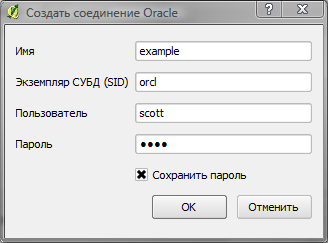
\includegraphics[clip=true, width=9cm]{oracle_create_dialog}
%\end{center}
%\end{figure}

\begin{figure}[ht]
\centering
   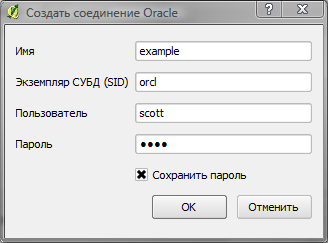
\includegraphics[width=7cm]{oracle_create_dialog}
   \caption{Fenêtre de création de connexion Oracle \nixcaption}\label{fig:oracle_create}
\end{figure}

%Now, back on the main Oracle Spatial GeoRaster dialog window (See Figure \ref{fig:oracle_select}), use the 
%drop-down list to choose one connection, and use the \button{Connect} button to establish a connection. You 
%may also \button{Edit} the connection by opening the previous dialog and making changes to the connection 
%information, or use the \button{Delete} button to remove the connection from the drop-down list.

(See Figure \ref{fig:oracle_select})
\button{Connecter} 
\button{Editer}
\button{Effacer}

\subsection{Sélection d'un GeoRaster}

%Once a connection has been established, the sub-datasets window will show the names of all the tables that 
%contains GeoRaster columns in that database in the format of a GDAL subdataset name.

Une fois que la connexion a été établie, la zone de sous-jeux de données affichera toutes les tables contenant une colonne GeoRaster dans un format compatible avec GDAL.

%Click on one of the listed subdatasets and then click on \button{Select} to choose the table name. Now another 
%list of subdatasets will show with the names of GeoRaster columns on that table. This is usually a short list, 
%since most users will not have more than one or two GeoRaster columns on the same table.

Cliquez sur l'un de ces sous-jeux de données puis sur \button{Sélectionner} pour choisir la table. Une nouvelle liste affiche maintenant les noms des colonnes GeoRaster dans cette table, il s'agit généralement d'une courte liste car la plupart des utilisateurs n'ont pas plus d'une ou deux colonnes GeoRaster dans une même table.

%Click on one of the listed subdatasets and then click on \button{Select} to choose one of the the table/column 
%combination. The dialog will now show all the rows that contains GeoRaster objects. Note that the subdataset 
%list will now show the Raster Data Table and Raster Id's pairs.

Cliquez sur l'une des sous-jeux puis sur \button{Sélectionner} pour choisir une combinaison d'une table et d'une colonne La fenêtre montrera alors toutes les lignes contenant un objet GeoRaster Vous remarquerez que la liste affichera la table de données raster et les identifiants Raster

%At anytime the Selection entry can be edited in order to go directly to a known GeoRaster or to go back to the 
%beginning and select another table name.

A tout moment la sélection peut être éditée manuellement pour pointer directement le Georaster voulu ou retourner au début pour prendre une autre table.

\begin{figure}[ht]
\centering
   
   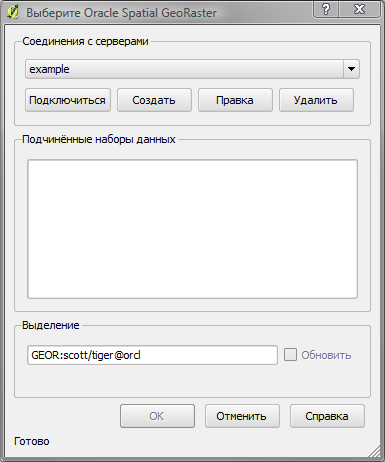
\includegraphics[clip=true, width=9cm]{oracle_select_dialog}
   \caption{Dialogue de sélection GeoRaster \nixcaption}\label{fig:oracle_select}
\end{figure}

%The Selection data entry can also be used to enter a Where clause at the end of the  identification string, e.g., 
%``geor:scott/tiger@orcl,gdal\_import,raster,geoid=''. See \url{http://www.gdal.org/frmt_georaster.html} for more information.

La zone de saisie de sélection peut servir à utilier une clause Where à la fin de la chaîne d'identification, p. ex. ``geor:scott/tiger@orcl,gdal\_import,raster,geoid=''. Voir \url{http://www.gdal.org/frmt_georaster.html} pour plus d'informations.

%\subsection{Displaying GeoRaster}
\subsection{Afficher un GeoRaster}

Pour finir, en sélectionnant un GeoRaster depuis la liste, cette image sera chargée dans \qg.

%The Select Oracle Spatial GeoRaster dialog window can be closed now and next time it opens it will keep the same 
%connection, and will show the same previous list of subdataset making it very easy to open up another image 
%from the same context.

La fenêtre de sélection de GeoRaster Oracle Spatial peut maintenant être close, la connnexion sera conservée pour une prochaine ouverture, la même liste de sous-jeux de donnéessera disponible ce qui facilite l'affichage de nouvelles images dans le même contexte.

/%\textbf{Note:} GeoRasters that contains pyramids will display much faster but the pyramids need to be generated 
%outside of \qg using Oracle PL/SQL or gdaladdo.
textbf{Note:} Les GeoRasters qui contiennent des tuiles/pyramides s'afficheront plus rapidement mais elles devront être générées hors de \qg en utilisant Oracle PL/SQL ou gdaladdo.

%The following is example using gdaladdo:
L'exemple suivant utilise gdaladdo :
\begin{verbatim}
gdaladdo georaster:scott/tiger@orcl,georaster\_table,georaster,georid=6 -r 
nearest 2 4 6 8 16 32
\end{verbatim}

Cet exemple utilise PL/SQL: 
cd ..
\begin{verbatim}
$ sqlplus scott/tiger
SQL> DECLARE
    gr sdo_georaster;
BEGIN
    SELECT image INTO gr FROM cities WHERE id = 1 FOR UPDATE;
    sdo_geor.generatePyramid(gr, 'rLevel=5, resampling=NN');
    UPDATE cities SET image = gr WHERE id = 1;
    COMMIT;
END;
/
\end{verbatim}
